\input ../SlidePreamble
\input ../preamble


\begin{document}

{\Huge
  \centerline{\bf TTIC 31230,  Fundamentals of Deep Learning}
  \vfill
  \centerline{David McAllester, Winter 2020}
  \vfill
  \centerline{\bf Contrastive Predictive Coding}
  \vfill
  \vfill
  
\slide{Contrastive Predictive Coding (CPC)}

We consider a population distribution on pairs $\tuple{x,y}$.

\vfill
For example $x$ and $y$ might be video frames separated by 10 seconds in a video.

\vfill
For simplicity we will assume that the marginal distributions on $x$ and $y$ are the same --- the probability that an image occurs as a first frame
is the same as the probability that image occurs as a second frame.

\vfill
In CPC we draw a pair $\tuple{x,y}$ and {\color{red} minimize} a discriminator loss for distinguishing $z_\Phi(y)$ from $z_\Phi(\tilde{y})$ for $\tilde{y} \sim \pop(y)$.
The discriminator gets to see $x$.

\slide{Contrastive Predictive Coding (CPC)}

For $N \geq 2$ let  $\tilde{P}^{(N)}$ be the distribution on tuples $\tuple{i,y_1,\ldots,y_N,x}$
defined by the following process.

\begin{itemize}
\item draw a pair $\tuple{x,y}$ from the population.

\item drawn a sequence of $N-1$ ``distractor values'' from the marginal distribution $\pop(y)$.  These are unrelated to $x$.

\item insert $y$ at a random position among the distractors to get the sequence
$y_1,\ldots,y_N$.

\item return the tuple $\tuple{i,y_1,\ldots,y_N,x}$ where $i$ is the index of $y$ among the distractors.
\end{itemize}

\slide{Contrastive Predictive Coding (CPC)}

\begin{eqnarray*}
\Phi^*  & = & \argmin_\Phi\;{\cal L}_\mathrm{CPC}(\Phi) \\
\\
{\cal L}_\mathrm{CPC}(\Phi) &= & E_{\tuple{i,y_1,\ldots,y_N,x} \sim \tilde{P}^{(N)}} \\
\\
& & ~\;\;\;\;\;\; -\ln P_\mathrm{CPC}(i|z_\Phi(y_1),\ldots,z_\Phi(y_N),z_\Phi(x))
\end{eqnarray*}

\vfill
$$P_\mathrm{CPC}(i|z_1,\ldots,z_N,z_x) = \softmax_i\;z_i^\top z_x$$

\slide{Contrastive Predictive Coding (CPC)}

\begin{eqnarray*}
\Phi^*  & = & \argmin_\Phi\;{\cal L}_\mathrm{CPC}(\Phi)
\end{eqnarray*}

\vfill
$$P_\Phi(i|z_1,\ldots,z_n,z_x) = \softmax_i\;z_i^\top z_x$$

\vfill
As $N$ gets larger the contrastive discrimination task gets harder.

\vfill
The task is also made difficult by the requirement that the score is defined to be an inner product of feature vectors.

\slide{Contrastive Predictive Coding (CPC)}

(SimCLR:) A Simple Framework for Contrastive Learning of Visual Representations, Chen et al., Feb. 2020 (self-supervised leader as of February, 2020).

\vfill
They use a distribution on pairs $\tuple{x,y}$ defined by drawing an image $s$ from ImageNet and then drawing $x$ and $y$ as random ``augmentations'' (modifications) of the image $s$
--- either a random translation, rotation, color jitter, masking, edge image, or a composition of these modifications.

\slide{Contrastive Predictive Coding (CPC)}

The feature map $z_\Phi$ can then be applied to the images of ImageNet.

\vfill
The feature map $z_\Phi$ is then tested by using a {\color{red} linear} classifier for ImageNet based on these features.

\slide{SimCLR}

\centerline{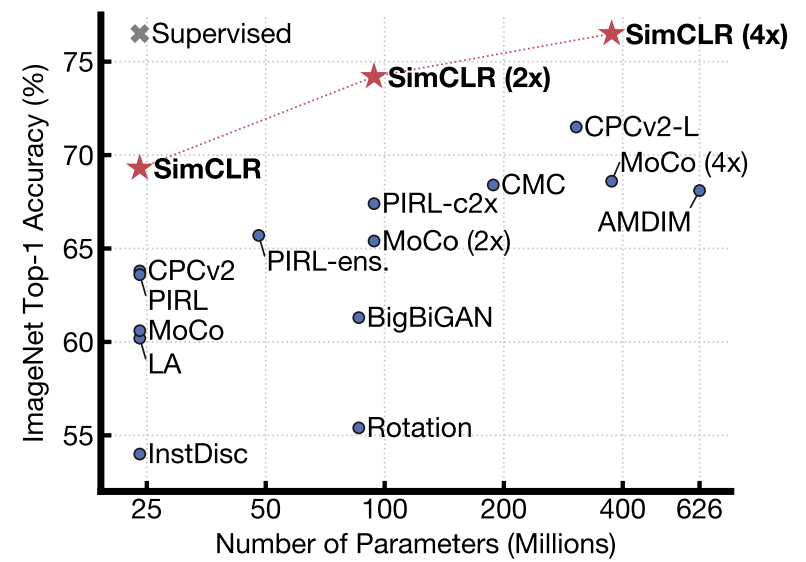
\includegraphics[height=5.2 in]{\images/SimCLR}}

\slide{END}

}
\end{document}
